\documentclass[12pt]{article}
\usepackage{indentfirst}
\usepackage{amsmath}
\usepackage{multicol}
\setlength{\jot}{2ex}
\usepackage{mathrsfs}
\usepackage{graphicx}
\usepackage{wrapfig}
\usepackage{booktabs}
\usepackage[letterpaper, margin=1in]{geometry}
\usepackage{fancyhdr}
\usepackage{enumitem}
\usepackage [autostyle, english = american]{csquotes}
\MakeOuterQuote{"}
\renewcommand{\baselinestretch}{1.0}
\newcommand{\objects}[2]{%
  \leavevmode\vbox{\hbox{#1}\nointerlineskip\hbox{#2}}%
}
\begin{document}
    \begin{titlepage}
        \begin{center}
            \textbf{Qadis Chaudhry} \\
            \vspace{0.2cm}
            202001055 \\
            \vfill
            \textbf{Project \#1} \\
            \vspace{0.2cm}
            October 11, 2021 \\
            \vfill
            Principles of Electrical Engineering II 332:222 \\
            \vspace{0.2cm}
            Fall 2021
        \end{center}
    \end{titlepage}
    \section*{Introduction}
    \par So far in this course we have examined three separate types of
    circuits, the RC, RL, and RLC configurations. For the tasks of this project
    we will focus on RC circuits, which contain resistors and one capacitor.
    The resistor is a simple passive device which does not possess the ability
    to store energy, it can only dissipate it. The capacitor on the other hand
    is an energy storing device, as it stores charge, and its equations reflect
    that by being time dependent. Ohm's Law is able to define the behavior of a
    resistor quite simply with a time invariant linear relationship, however,
    the behavior of the capacitor will vary with respect to time. Conceptually,
    to understands this we can examine a parallel plate capacitor with current
    flowing into one end.
    \par As the current flows into one of the plates of the capacitor, electrons
    will flow into and deposit onto the plate. Since the plates of the capacitor
    are separated by some distance, there will be nowhere for the electrons to
    go and they must deposit on the face of the plate. Current can be defined as
    the flow of change per unit of time and for this reason, as time goes on
    there will be more and more charge that accumulates on the plate. The
    principle that like charges repel will dictate it becoming increasingly
    difficult to deposit more charge, causing the flow rate of charge to keep
    decreasing over time. This will be seen in the math as a decaying
    relationship between the current that flows into and the voltage that is
    across the capacitor.
    \par With this basic concept in mind, as we look at the RC circuit, we can
    see how the equation to describe the configuration will be differential and
    of the first order. There are two cases which are common to observe with
    these circuits, the natural and the step response. The natural response
    occurs when there is no source connected and therefore the capacitor holds
    all the voltage and it is dissipated by the resistor. On the other hand, we
    have the step response, which is akin to the charging of the capacitor. This
    charging and discharging can be linked together with the equations, and are
    useful to understand in the analysis of large scale circuits which possess
    both responses.
    \section*{Task 1}
    \begin{figure}[h]
        \centering
        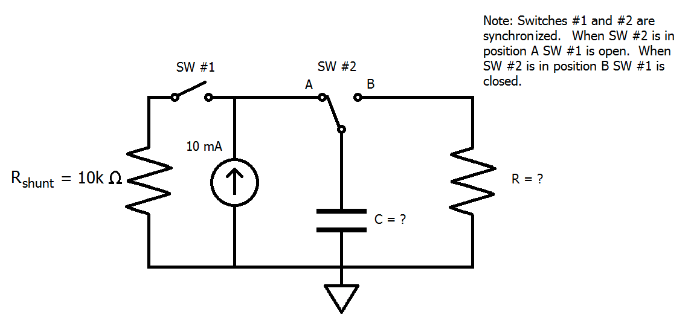
\includegraphics[width=0.67\textwidth]{Task 1 Schematic.png}
        \caption{Circuit Schematic}
    \end{figure}
    \begin{figure}[h]
        \centering
        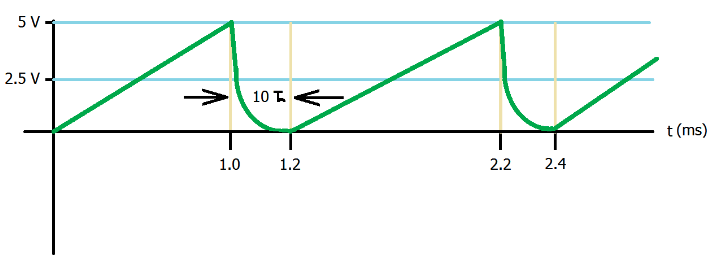
\includegraphics[width=0.8\textwidth]{Task 1 Waveform.png}
        \caption{Waveform}
    \end{figure}
    \textbf{Task:} Calculate the values of $C$ and $R$ needed to produce
    the waveform shown above.
    \subparagraph*{} In order to find the value of $C$ we can employ the equation relating
    the current and voltage in a capacitor,
    \[
        i(t) = C\ \frac{dv}{dt}
    \]
    For the 1 millisecond that switch 2 is in position A, the circuit is
    simplified to a capacitor connected to a current source.  Since the current
    source has a constant value of 10 mA, the expression for $i(t)$ is constant
    and does not change over time $t$. Along with this, from the graph of the
    waveform, the slope of the linear rise can be found to be $\frac{5 - 0}{1
    \times 10^{-3} - 0}$ from $t=0$ ms to $t=1$ ms. This is the value of
    $\frac{dv}{dt}$ in the equation since the derivative of voltage would be its
    rate of change with respect to time, the slope of $v$ vs. $t$.  From here,
    we can plug into the equation where $C$ is the only unknown,
    \[
        10 \times 10^{-3} = C \left( \frac{5}{1 \times 10^{-3}} \right)
    \]
    Solving for $C$ we get,
    \[
        C = \frac{(1 \times 10^{-3})(10 \times 10^{-3})}{5} = 2 \times 10^{-6} = \boxed{2\ \mu F}
    \]
    \par Now for the value of the resistor. We can see from the waveform that
    the value of time for which switch 2 is in position B, 0.2 ms, is equivalent
    to 10$\tau$, where $\tau$ is the time constant. Since this is an RC circuit,
    the value of $\tau$ is given by $R$ multiplied by $C$, and since we have the
    value of $C$, we can find $R$.
    \begin{alignat*}{2}
        \tau &\,=\, \, \, \frac{0.2 \times 10^{-3}}{10} &&\,=\, 2 \times 10^{-5} = RC \\
        RC &\,=\, R(2\times 10^{-6}) &&\,=\, 2 \times 10^{-5} \\
        R &\,=\quad \frac{2 \times 10^{-5}}{2 \times 10 ^{-6}} &&\,=\, \boxed{10 \Omega}
    \end{alignat*}
    \newpage
    \section*{Task 2}
    \begin{figure}[h]
        \centering
        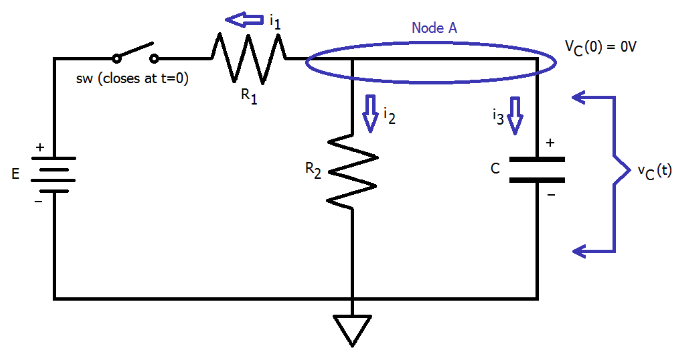
\includegraphics[width=0.7\textwidth]{Task 2 Schematic.png}
        \caption{Circuit Schematic}
    \end{figure}
    \textbf{Task:} Derive the general formula for $v_{c}(t)$ for $t \ge 0$ in
    terms of the given variables.
    \subparagraph*{} This circuit will yield the step response of an RC circuit
    since at time $t = 0$, the switch closes and the voltage source is connected
    to the circuit. Since the switch has been open for a long time, the initial
    conditions for voltage and current are zero,
    \[
        v(0) = 0,\ i(0) = 0.
    \]
    At node A, we can sum together the currents and set them equal to zero since
    according to KCL and nodal analysis, the sum of all currents going into or
    out of a node must equal zero.
    \[
        i_1 + i_2 + i_3 = 0.
    \]
    To define each of these currents we can see that node A will be at a
    voltage, $v_{c}$. In addition, $i_3$ is simply the current through the
    capacitor which can be related by the equation $C\frac{dv_{c}}{dt}$. Using
    this information, $i_1 = \frac{v_{c} - E}{R_1}$, $i_2 =
    \frac{v_{c}}{R_{2}}$, and $i_3 = C \frac{dv_{c}}{dt}$. We can now plug these
    currents into the equation and begin solving for $v_{c}$.
    \[
        \frac{v_{c} - E}{R_1} + \frac{v_{c}}{R_{2}} + C\ \frac{dv_{c}}{dt} = 0.
    \]
    To get the derivative term by itself, we can divide the equation by $C$ and
    rearrange to get this into the standard form for a linear ordinary
    differential equation.
    \begin{align*}
        \frac{dv_{c}}{dt} + \frac{v_{c} - E}{R_1C} + \frac{v_{c}}{R_2C} &= 0 \\
        \frac{dv_{c}}{dt} + \left( \frac{1}{R_1C} + \frac{1}{R_2C} \right)v_{c} &= \frac{E}{R_1C} \\
        v_{c}' + \left( \frac{1}{R_1C} + \frac{1}{R_2C} \right)v_{c} &= \frac{E}{R_1C}
    \end{align*}
    This equation can be solved as any other linear ODE with the use of the
    integration factor, $e^{\int p(t) dt}$. Here, we will define it as $\mu$.
    \begin{align*}
        p(t) &= \left( \frac{1}{R_1C} + \frac{1}{R_2C} \right) = \delta \\
        \int p(t)\ dt &= \left( \frac{1}{R_1C} + \frac{1}{R_2C} \right)t = \delta t \\
        \mu &= e^{\left( \frac{1}{R_1C} + \frac{1}{R_2C} \right)t} = \mu^{\delta t}
    \end{align*}
    Since $p(t)$ here has a constant value, we will call it delta to clear up the
    derivation. The equation can then be written as,
    \begin{align*}
        \left( \mu v_{c} \right)' &= \mu \frac{E}{R_1C} \\
        v_{c}e^{\delta t} &= \frac{E}{R_1C} \int e^{\delta t}\ dt
    \end{align*}
    Solving the integral and isolating the term $v_{c}$,
    \begin{align*}
        v_{c}(t) &= \frac{E}{R_1C}\ e^{-\delta t} \left( \frac{1}{\delta} e^{\delta t} + k \right) \\
        v_{c}(t) &= \frac{E}{R_1C} \left( \frac{1}{\delta} + ke^{-\delta t} \right)
    \end{align*}
    Here, $k$ is the arbitrary constant of integration and can be solved for
    plugging in the initial condition, $v_{c}(0) = 0$,
    \[
        0 = \frac{E}{R_1C} \left( \frac{1}{\delta} + ke^{0} \right)
    \]
    and since $e^{0} = 1$,
    \[
        k = -\frac{1}{\delta}
    \]
    With that, the capacitor voltage can be written by substituting in the
    expression for delta and rearranging, and the derivation is finished.
    \begin{align*}
        v_{c}(t) &= \frac{E}{R_1C} \left( \frac{1}{\delta} - \frac{1}{\delta}e^{-\delta t} \right) \\
        v_{c}(t) &= \frac{E}{R_1C} \frac{1}{\delta} \left( 1 - e^{-\delta t} \right)
    \end{align*}
    \[
        v_{c}(t) = \frac{E}{R_1C} \left( \frac{1}{R_1C} + \frac{1}{R_2C}
        \right)^{-1} \left( 1 - e^{-\left( \frac{1}{R_1C} + \frac{1}{R_2C}
        \right)t} \right)
    \]
    \[
        \boxed{v_{c}(t) = \frac{ER_2}{R_1 + R_2} \left( 1 - e^{-\left( \frac{R_1 +
        R_2}{R_1R_2C} \right)t} \right)}
    \]
\end{document}
